\documentclass{exam}
\usepackage{../../mypackages}
\usepackage{../../macros}

\title{Interro N°1 - Chimie organique}
\author{N. Bancel}
\date{Novembre 2024}

\begin{document}

\textbf{Collège Lycée Suger}
\hfill
\textbf{Physique-Chimie} \\

\textbf{Année 2024-2025}
\hfill
\textbf{1ères STD2A} \par

{\let\newpage\relax\maketitle}

\begin{center}
\textbf{\textcolor{red}{Durée : 30 minutes. La calculatrice n'est pas autorisée}} \\
\textbf{\textcolor{red}{Une réponse donnée sans justification sera considérée comme fausse.}} \\

\end{center}

\section*{Partie 1 : Cours sur les hydrocarbures (6.5 points)}

\begin{questions}
  \question[1] Sachant que le numéro atomique de l'atome de Carbone est $Z=6$, justifier pourquoi il a 4 doublets non-liants

  \question[1] Donner la définition
  \begin{parts}
    \part[0.5] D'un alcane
    \part[0.5] D'un alcène
\end{parts}

\question[1] Identifier les familles de composés associées aux groupes caractéristiques suivants

\begin{figure}[H]
    \centering
    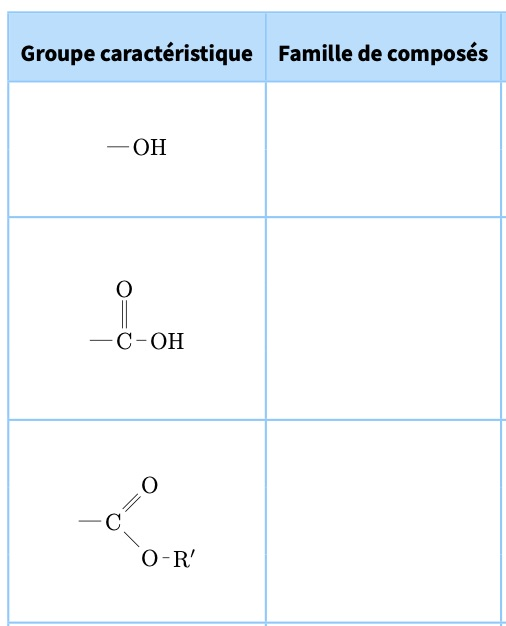
\includegraphics[width=0.4\linewidth]{interro1_01.jpg}
    \caption{Polymérisation}
\end{figure} 

\question[3.5] Compléter le tableau ci-dessous 

\begin{center}
\begin{tabular}{|| >{\centering\arraybackslash}p{2cm} | >{\centering\arraybackslash}p{5cm} | >{\centering\arraybackslash}p{3cm} | >{\centering\arraybackslash}p{4cm} ||}
  \toprule
  {Formule brute} & {Formule developpée} & {Formule semi-développée} & {Formule topologique} \\
  \midrule
  {...} & {\chemfig{H-C(-[2]H)(-[6]H)-C(-[2]H)(-[6]H)-C(-[2]H)(-[6]H)-H}} & {...} & {...} \\ [4em]
  {\ce{C2H6}} & {...} & {...} & {...} \\[4em]
  {...} & {...} & {\ce{CH3-COOH}} & {...} \\[4em]
  {...} & {...} & {...} & {\chemfig{[:30]--[:-30]-([:30]OH)}} \\[4em]
  {...} & {...} & {...} & {\chemfig{HO-[:-45](-[:-135])-[:0](=[:-45]O)(-[:45])}} \\[4em]
  \bottomrule
\end{tabular}
\end{center}

\end{questions}

\section*{Partie 2 : Les polymères (3.5 points)}

\begin{questions}

\question[3.5] Le polyamide 11, appelé aussi "nylon français" ou nylon 11, est un polymère thermoplastique bio-sourcé utilisé pour fabriquer des cordes d'instruments de musique ou des conduites flexibles pour les secteurs pétroliers. Sa synthèse est donnée par la réaction ci-dessous :

\begin{figure}[H]
  \centering
  
\includegraphics[width=0.6\linewidth]{interro1_02.jpg}
  \caption{Groupes caractéristiques}
\end{figure} 

\begin{parts}
  \part[0.5] Definir le terme "biosourcé"
  \part[0.5] Repérer le motif du nylon 11 et en donner la formule brute 
  \part[0.5] Repérer le groupe caractéristique apparaissant dans le motif du nylon français et donner la famille de composés associée.
  \part[0.5] Repérer les autres groupes caractéristiques apparaissant dans cette réaction et donner les familles de composés associées
  \part[0.5] Le polyamide 11 est-il synthétisé par polyaddition ou polycondensation ?
  \part[1] Qu'est ce qu'un polymère et qu'est ce signifie l'indice de polymérisation ? 
\end{parts}

\end{questions}

\section*{Aides}


Voici d'autres groupes caractéristiques et leur famille de composés : 





\begin{center}
  \begin{tabular}{|| >{\centering\arraybackslash}p{4cm} | >{\centering\arraybackslash}p{5cm} | >{\centering\arraybackslash}p{3cm} ||}
    \toprule
    {Groupe caractéristique} & {Famille de composés} & {Formule générale} \\
    \midrule
    {\ce{-NH2}} & {Amine primaire} & {\ce{R-NH2}}  \\ [4em]
    {\chemfig{-C(=[1]O)-[7]N-}} & {Amide} & {\ce{R1-CO-NH-R2}} \\ [4em]

    \bottomrule
  \end{tabular}
  \end{center}


\end{document}
